\documentclass[a4paper, 10pt]{article}
\usepackage{a4wide}
\usepackage{graphicx}
\usepackage{listings}
\usepackage{color}
\usepackage[usenames,dvipsnames]{xcolor}
\usepackage{verbatim}
\usepackage{fancyhdr}
\usepackage{lastpage}
\pagestyle{fancy}

\fancyhead[LE,RO]{\textit{C++, C \& Java Programming Paradigms / Connor Goddard}}
\fancyhead[LO,RE]{\slshape}
\renewcommand{\headrulewidth}{0pt}

\fancyfoot[LE,RO]{Page \thepage\ of \pageref{LastPage}}
\cfoot{}


\lstdefinestyle{customc++}{
  belowcaptionskip=1\baselineskip,
  breaklines=true,
  frame=L,
  language=C++,
  showstringspaces=false,
  basicstyle=\footnotesize\ttfamily,
  keywordstyle=\bfseries\color{OliveGreen},
  commentstyle=\itshape\color{black},
  identifierstyle=\color{blue},
  stringstyle=\color{orange},
  numbers=left
}

\lstdefinestyle{customjava}{
  belowcaptionskip=1\baselineskip,
  breaklines=true,
  frame=L,
  language=Java,
  showstringspaces=false,
  basicstyle=\footnotesize\ttfamily,
  keywordstyle=\bfseries\color{OliveGreen},
  commentstyle=\itshape\color{black},
  identifierstyle=\color{blue},
  stringstyle=\color{orange},
  numbers=left
}

\lstdefinestyle{buildlog}{
  basicstyle=\scriptsize\ttfamily,
  breaklines=true,
  frame=L,
  showstringspaces=false,
  numbers=left
}

\lstdefinestyle{output}{
  basicstyle=\scriptsize\ttfamily,
  breaklines=true,
  frame=single,
  showstringspaces=false
}

\setlength{\parindent}{0pt}

\title{\textbf{CS22510 - C++, C \& Java Programming Paradigms} \\ Assignment 1 - Runners \& Riders \\ 2012-2013}	
\author{\textbf{Connor Luke Goddard}\\clg11@aber.ac.uk}		
\date{March 2013}	

\begin{document}

\begin{titlepage}
\maketitle
\thispagestyle{empty}
\end{titlepage}

\tableofcontents
\clearpage

\section{Introduction}

\subsection{Purpose of this Document}
The purpose of this document is to provide a description and supporting evidence of my implemented solution to the CS22510 Assignment 1. 

\subsection{Scope}
This document describes the final state of the implemented solution and contains  evidence demonstrating the functionality, compilation, and source code of all three applications that form to produce the final system.

\subsection{Objectives}

The objectives of this document are:

\begin{itemize}

\item To provide the complete source code for the ``event creator" application, and evidence of it's compilation and functionality.
\item To provide the complete source code for the ``checkpoint manager" application, and evidence of it's compilation and functionality.
\item To provide evidence of the compilation and functionality of the ``event manager" applicaiton.
\item To briefly describe the structure and programming language choice of each of the three applications.

\end{itemize}

\section{Design Assumptions}

To allow a definitive design for the checkpoint manager to be established, the following assumption has had to be drawn:

\begin{enumerate}

\item When logging new time values for \textbf{medical checkpoints}, a user will submit arrival and departure times \textbf{separatly} (i.e. separate transactions), and not at the same time. This will allow other entrant checkpoint time values to be logged while an entrant is waiting at a medcial checkpoint.

\end{enumerate}



\clearpage

\section{Event Creator (C++) - Source Code}

This section contains the complete source code for the ``event creator" program written in C++.

\subsection{Header Files}

\subsubsection{Menu.h}
\lstinputlisting[style=customc++]{../Event-Creator/Menu.h}

\clearpage
\subsubsection{Process.h}
\lstinputlisting[style=customc++]{../Event-Creator/Process.h}

\clearpage
\subsubsection{Datastore.h}
\lstinputlisting[style=customc++]{../Event-Creator/Datastore.h}

\clearpage
\subsubsection{FileIO.h}
\lstinputlisting[style=customc++]{../Event-Creator/FileIO.h}

\clearpage
\subsubsection{Event.h}
\lstinputlisting[style=customc++]{../Event-Creator/Event.h}

\clearpage
\subsubsection{Entrant.h}
\lstinputlisting[style=customc++]{../Event-Creator/Entrant.h}

\clearpage
\subsubsection{Node.h}
\lstinputlisting[style=customc++]{../Event-Creator/Node.h}

\clearpage
\subsubsection{Course.h}
\lstinputlisting[style=customc++]{../Event-Creator/Course.h}

\clearpage
\subsection{Class Files}

\subsubsection{Main.cpp}
\lstinputlisting[style=customc++]{../Event-Creator/main.cpp}

\clearpage
\subsubsection{Menu.cpp}
\lstinputlisting[style=customc++]{../Event-Creator/Menu.cpp}

\clearpage
\subsubsection{Process.cpp}
\lstinputlisting[style=customc++]{../Event-Creator/Process.cpp}

\clearpage
\subsubsection{Datastore.cpp}
\lstinputlisting[style=customc++]{../Event-Creator/Datastore.cpp}

\clearpage
\subsubsection{FileIO.cpp}
\lstinputlisting[style=customc++]{../Event-Creator/FileIO.cpp}

\clearpage
\subsubsection{Event.cpp}
\lstinputlisting[style=customc++]{../Event-Creator/Event.cpp}

\clearpage
\subsubsection{Entrant.cpp}
\lstinputlisting[style=customc++]{../Event-Creator/Entrant.cpp}

\clearpage
\subsubsection{Node.cpp}
\lstinputlisting[style=customc++]{../Event-Creator/Node.cpp}

\clearpage
\subsubsection{Course.cpp}
\lstinputlisting[style=customc++]{../Event-Creator/Course.cpp}

\clearpage
\section{Event Creator - Build/Compilation Log}

The listing below contains the build/compilation log for the ``event creator" application. Extra warning flags have been used with the C++ compiler (\textbf{g++}) to ensure that no errors/warnings occur when compiling the application.

\lstinputlisting[style=buildlog, caption=Compilation log built within Netbeans IDE 7.3 on Ubuntu 12.04]{event-creator-buildlog.txt}

\clearpage
\section{Event Creator - Example Usage}
This section demonstrates the ``event creator" application running using test input data to ensure that expected functionality and suitable error checking is taking place correctly.

\lstinputlisting[style=output, caption=Example output of functionality testing of the event creator application.]{event-creator-output.txt}

\clearpage
\section{Event Creator - File Output}

This section lists the contents of the three external files that the event creator application has produced from the user input provided from the previous test run. 

\lstinputlisting[style=output, basicstyle=\footnotesize\ttfamily, caption=Output of `event.txt' file produced by the ``event creator" application.]{../files/exampleevent.txt}

\lstinputlisting[style=output, basicstyle=\footnotesize\ttfamily, caption=Output of `courses.txt' file produced by the ``event creator" application.]{../files/examplecourses.txt}

\lstinputlisting[style=output, basicstyle=\footnotesize\ttfamily, caption=Output of `entrants.txt' file produced by the ``event creator" application.]{../files/exampleentrants.txt}

\clearpage
\section{Checkpoint Manager (Java) - Source Code}
This section contains the complete source code for the ``checkpoint manager" program written in Java (JVM 7).

\subsection{`Driver' Package}

\subsubsection{CMDriver.java}
\lstinputlisting[style=customjava]{../Checkpoint-Manager/src/aber/dcs/cs22510/clg11/driver/CMDriver.java}

\clearpage
\subsection{`Util' Package}

\subsubsection{ProcessData.java}
\lstinputlisting[style=customjava]{../Checkpoint-Manager/src/aber/dcs/cs22510/clg11/util/ProcessData.java}

\clearpage
\subsubsection{FileIO.java}
\lstinputlisting[style=customjava]{../Checkpoint-Manager/src/aber/dcs/cs22510/clg11/util/FileIO.java}

\clearpage
\subsubsection{LoadData.java}
\lstinputlisting[style=customjava]{../Checkpoint-Manager/src/aber/dcs/cs22510/clg11/util/LoadData.java}

\clearpage
\subsection{`Model' Package}

\subsubsection{Datastore.java}
\lstinputlisting[style=customjava]{../Checkpoint-Manager/src/aber/dcs/cs22510/clg11/model/Datastore.java}

\clearpage
\subsubsection{Entrant.java}
\lstinputlisting[style=customjava]{../Checkpoint-Manager/src/aber/dcs/cs22510/clg11/model/Entrant.java}

\clearpage
\subsubsection{Course.java}
\lstinputlisting[style=customjava]{../Checkpoint-Manager/src/aber/dcs/cs22510/clg11/model/Course.java}

\clearpage
\subsubsection{Node.java}
\lstinputlisting[style=customjava]{../Checkpoint-Manager/src/aber/dcs/cs22510/clg11/model/Node.java}

\clearpage
\subsubsection{Datatype.java}
\lstinputlisting[style=customjava]{../Checkpoint-Manager/src/aber/dcs/cs22510/clg11/model/Datatype.java}

\clearpage
\subsection{`GUI' Package}

\subsubsection{GUIFrame.java}
\lstinputlisting[style=customjava]{../Checkpoint-Manager/src/aber/dcs/cs22510/clg11/gui/GUIFrame.java}

\clearpage
\subsubsection{GUIPanel.java}
\lstinputlisting[style=customjava]{../Checkpoint-Manager/src/aber/dcs/cs22510/clg11/gui/GUIPanel.java}

\clearpage
\section{Checkpoint Manager - Build/Compilation Log}

The listing below contains the build/compilation log for the ``checkpoint manager" application. Extra warning flags (\verb+-Xlint:unchecked+) have been used with the JVM compiler to ensure that no errors/warnings occur when compiling the application. \\

\lstinputlisting[style=buildlog, caption=Compilation log built within Netbeans IDE 7.3 on Ubuntu 12.04]{checkpoint-manager-buildlog.txt}

\clearpage
\section{Checkpoint Manager - Example Usage}
This section demonstrates the ``checkpoint manager" application running using test input data to ensure that expected functionality and suitable error checking is taking place correctly.\\

\subsection{Loading External Data Files}

\subsubsection{Correct File Parameters}

Parameter Input: \verb+"../files/nodes.txt" "../files/courses.txt" "../files/entrants.txt"+ \\\\
Output:
\lstinputlisting[style=output, caption=Textual output produced when correct file names are supplied.]{checkpoint-manager-output.txt}

\begin{figure}[ht!]
\centering
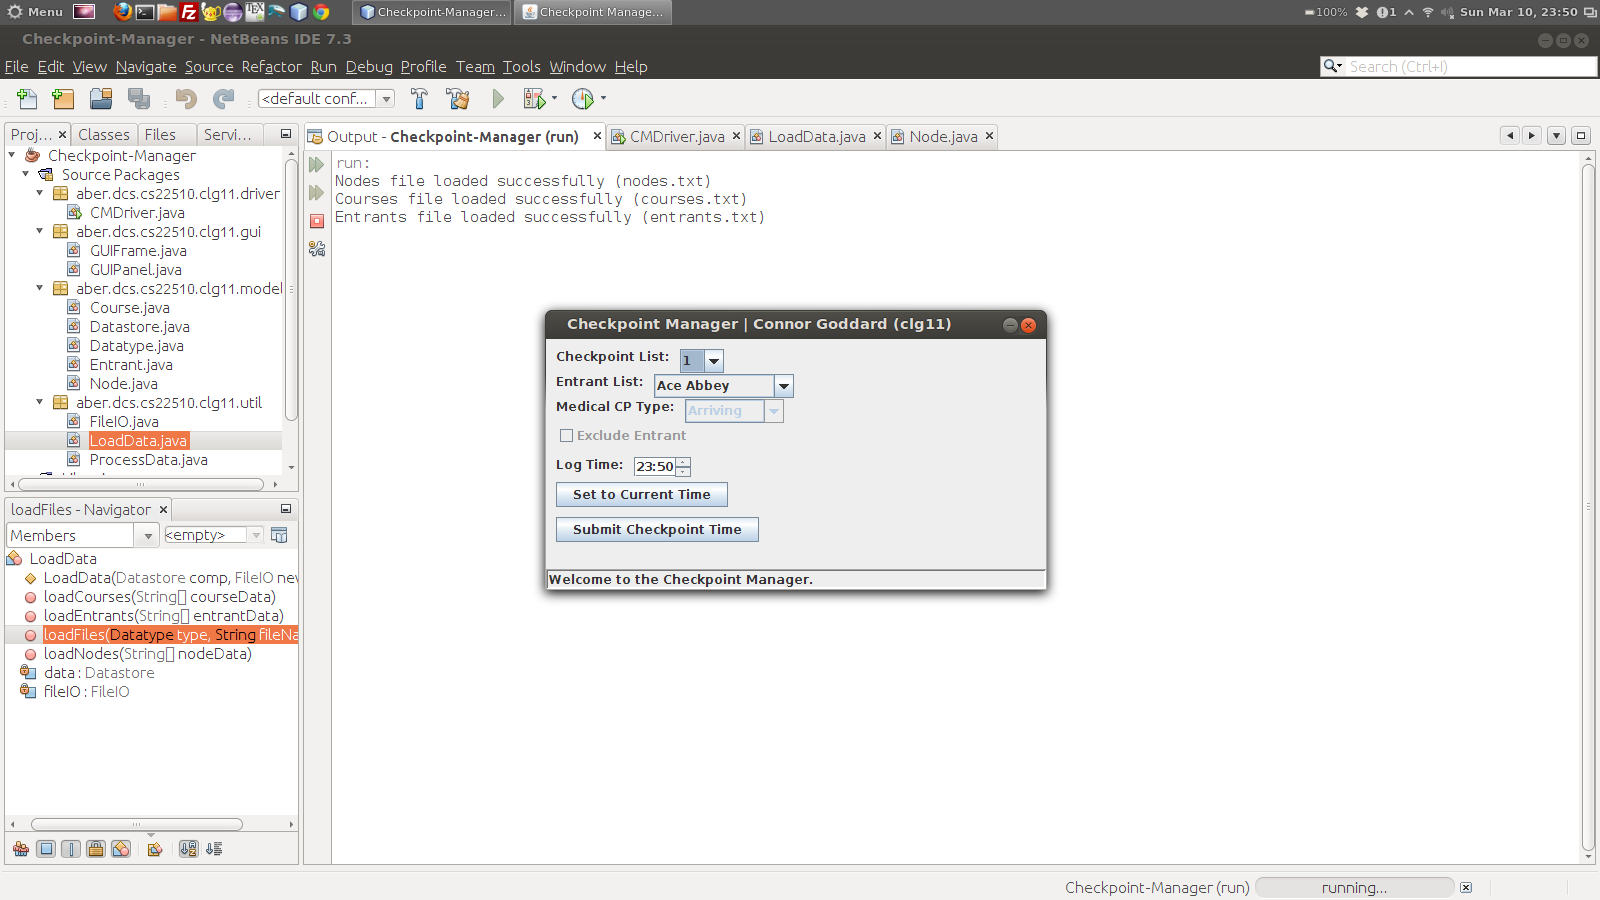
\includegraphics[scale=0.3]{cm-loadsuccess.png}
\caption{Screenshot displaying the GUI display after successfully loading the external data files.}
\end{figure}

\clearpage
\subsubsection{Incorrect File Parameters}

Parameter Input: \verb+"../files/nodes.txt" "../files/idontknow.txt" "../files/entrants.txt""+ \\\\
Output:
\lstinputlisting[style=output, caption=Textual warning output produced when incorrect file names parameters are supplied.]{checkpoint-manager-output-failure.txt}

\subsection{Submit Correct Time Entry}

Input: \verb+Entrant 1 - Checkpoint 1 (Starting checkpoint for course).+ \\
\begin{figure}[ht!]
\centering
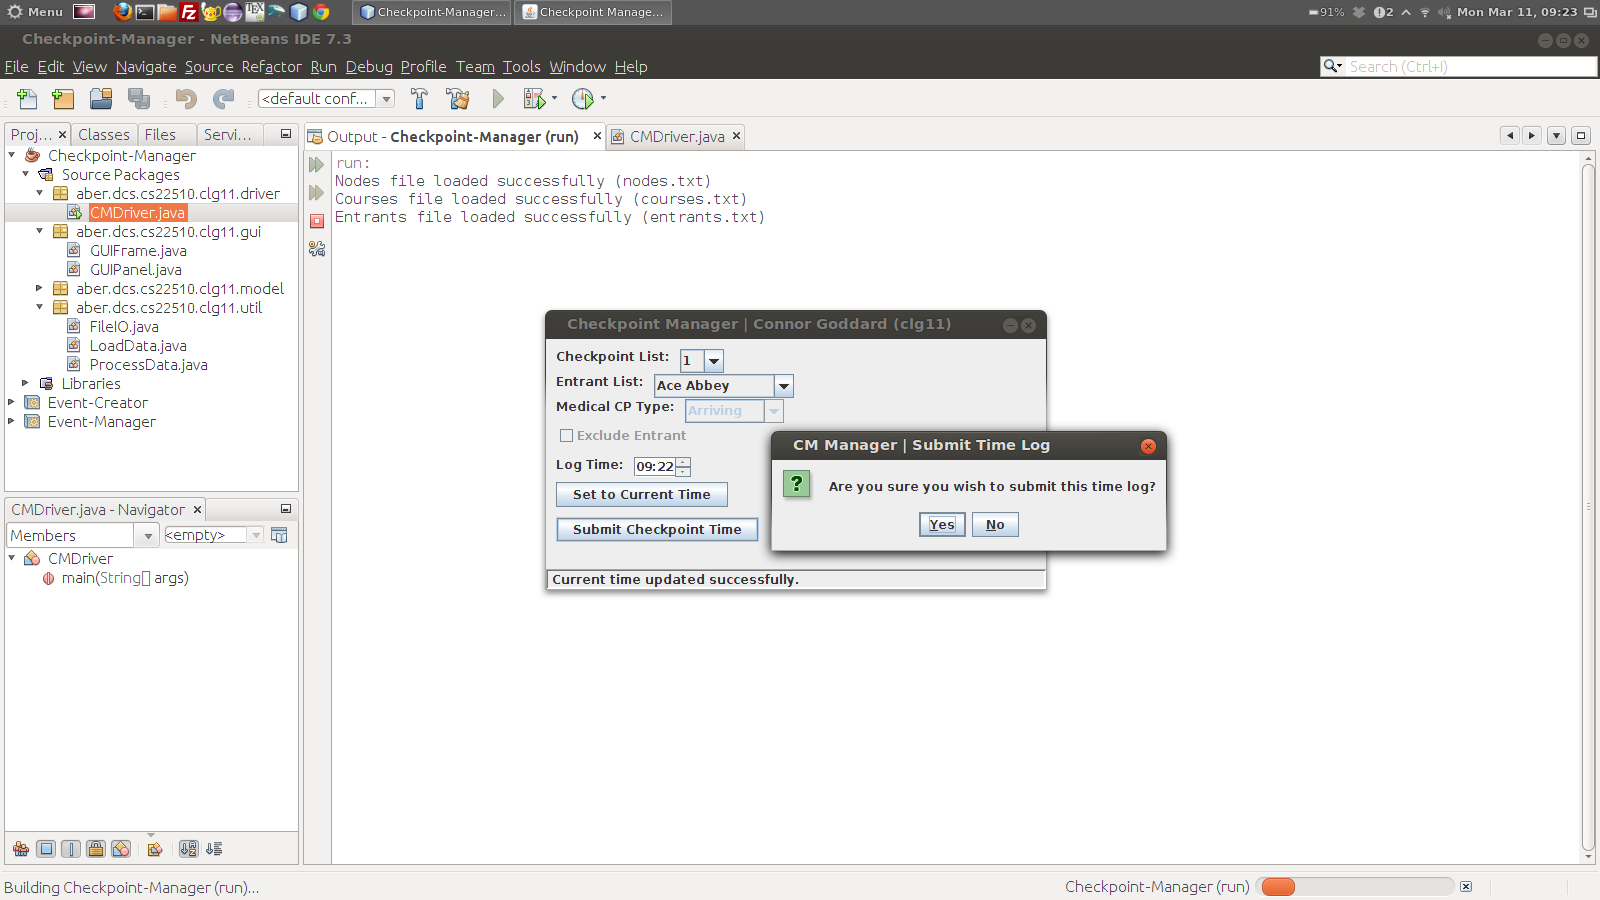
\includegraphics[scale=0.25]{cm-submit.png}
\caption{Screenshot displaying attempt to submit a correct time entry for an entrant.}
\end{figure}

Output:
\begin{figure}[ht!]
\centering
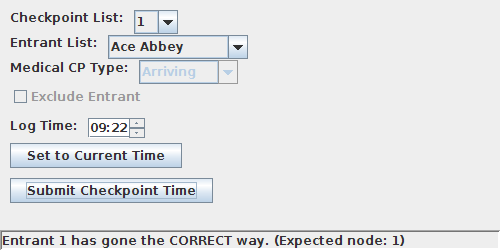
\includegraphics[scale=0.5]{cm-submitsuccess.png}
\caption{Checkpoint Manager GUI confirming successful submission of time entry.}
\end{figure}

\subsection{Submit Incorrect Time Entry}

Input: \verb+Entrant 3 - Checkpoint 4 (Incorrect - should be CP 1).+ \\

Output:
\begin{figure}[ht!]
\centering
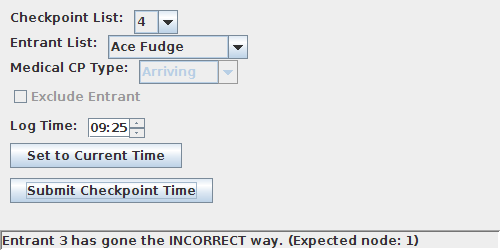
\includegraphics[scale=0.7]{cm-submitincorrect.png}
\caption{Checkpoint Manager GUI informing user that entrant has been logged at an incorrect checkpoint.}
\end{figure}

\subsection{Entrant Exclusion (Incorrect Node)}

Input: \verb+Entrant 3 - Checkpoint 1.+ \\

Output:
\begin{figure}[ht!]
\centering
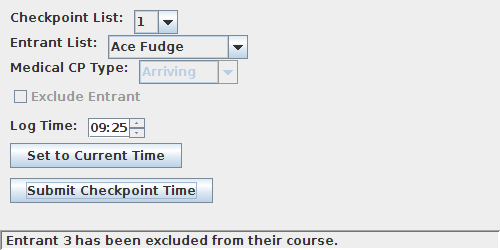
\includegraphics[scale=0.7]{cm-submitexclude.png}
\caption{Checkpoint Manager GUI informing user that entrant 3 has already been excluded from the event.}
\end{figure}

\clearpage
\subsection{Entrant Course Completion}

Input: \verb+Entrant 1 - Checkpoint 1 (After entrant has finished course).+ \\

Output:
\begin{figure}[ht!]
\centering
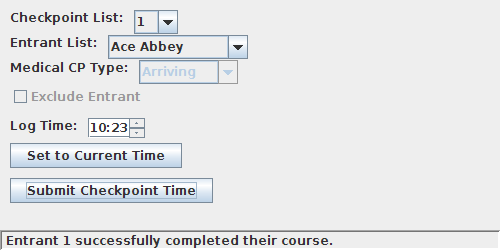
\includegraphics[scale=0.7]{cm-finished.png}
\caption{Checkpoint Manager GUI informing user that entrant 1 has successfully completed their course.}
\end{figure}

\subsection{Medical Checkpoint - Successful Arrival}

Input: \verb+Entrant 7 - MC 14 (Arriving).+ \\

Output:
\begin{figure}[ht!]
\centering
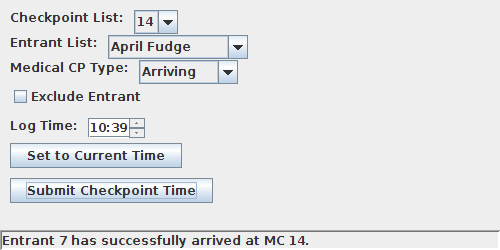
\includegraphics[scale=0.7]{cm-mcarrivesuccess.png}
\caption{Checkpoint Manager GUI informing user that entrant 7 has successfully arrived (correctly) at medical checkpoint 14.}
\end{figure}

\clearpage
\subsection{Medical Checkpoint - Successful Departure}

Input: \verb+Entrant 64 - MC 14 (Departing).+ \\

Output:
\begin{figure}[ht!]
\centering
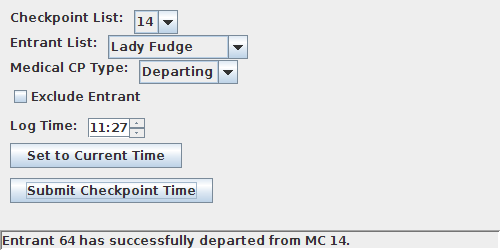
\includegraphics[scale=0.7]{cm-mcdepartsuccess.png}
\caption{Checkpoint Manager GUI informing user that entrant 64 has successfully departed (correctly) from medical checkpoint 14.}
\end{figure}

\subsection{Medical Checkpoint - Incorrect Arrival}

Input: \verb+Entrant 7 - MC 14 (Arriving - Already at MC 14).+ \\

Output:
\begin{figure}[ht!]
\centering
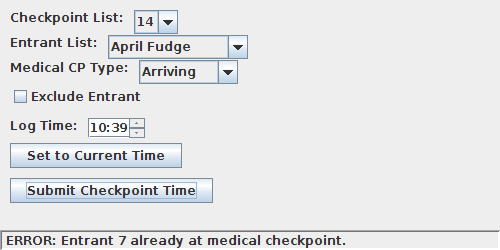
\includegraphics[scale=0.7]{cm-mcarrivefailure.png}
\caption{Checkpoint Manager GUI informing user that entrant 7 is already logged at MC 14 and so cannot have arrived again.}
\end{figure}

\clearpage
\subsection{Medical Checkpoint - Incorrect Departure}

Input: \verb+Entrant 98 - MC 14 (Departing - Entrant yet to begin course).+ \\

Output:
\begin{figure}[ht!]
\centering
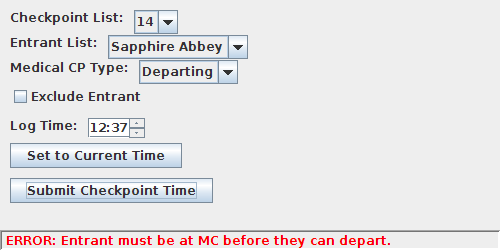
\includegraphics[scale=0.7]{cm-mcdepartfailure.png}
\caption{Checkpoint Manager GUI informing user that entrant 98 must have arrived at a MC before they can depart.}
\end{figure}

\subsection{Entrant Exclusion (Medical Reasons)}

Input: \verb+Entrant 7 - MC 14.+ \\

Output:
\begin{figure}[ht!]
\centering
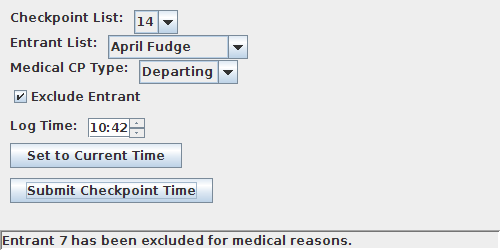
\includegraphics[scale=0.7]{cm-mcexclude.png}
\caption{Checkpoint Manager GUI informing user that entrant 7 has been successfully excluded for medical reasons.}
\end{figure}

\clearpage
\subsection{Submission of Invalid Time Value}

Input: \verb+Submitted Time: 08:46. Latest Logged Time: 09:37.+ \\

Output:
\begin{figure}[ht!]
\centering
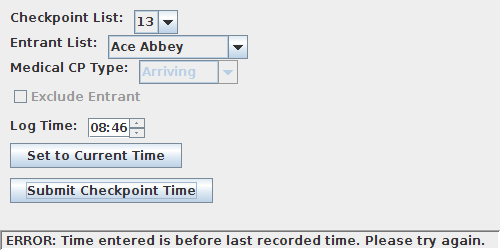
\includegraphics[scale=0.7]{cm-timesubmitfailure.png}
\caption{Checkpoint Manager GUI informing user that submitted time cannot be before the latest logged time (\textbf{Ensures time log file remains sequential}).}
\end{figure}

\subsection{System Activity Logging}

Input:\\\\
\verb+Variety of system activity. (Correct/incorrect node submissions,+\\
\verb+automatic loading of data files etc...)+\\

Output:
\lstinputlisting[style=output, caption=Example of log file produced by CM application of activity detailed above.]{cm-log.txt}

\clearpage
\subsection{File Lock Access Prevention}

Input:\\\\
\verb+Two instances of the Checkpoint Manager application deployed.+ \\\\
\verb+One application modified to prevent the release of the file lock.+\\

\begin{lstlisting}[style=customjava, caption=File export code modified to prevent a file lock being released once accessed.]
  //Check if the lock was successfull.
            if (fl != null) {

                try (FileWriter fw = new FileWriter(fos.getFD())) {

                    fw.write(output);

                    //Once the data has been successfully written, release the lock.
                    
                    //FILE LOCK RELEASE PREVENTED.
                    //fl.release();
                }

                return true;

            }

\end{lstlisting}

Output:
\begin{figure}[ht!]
\centering
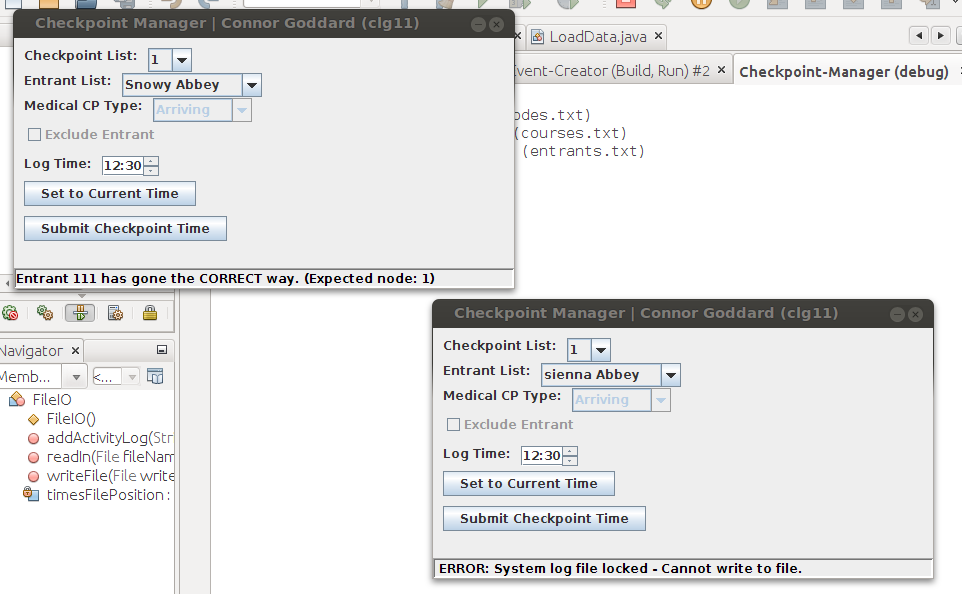
\includegraphics[scale=0.65]{cm-filelock.png}
\caption{Screenshot demonstrating modified CM application (top-left) preventing original CM application (bottom-right) from accessing log file ``log.txt".}
\end{figure}

\clearpage
\subsection{Entrant Times File Generation}

This sub-section contains the times file (``times.txt") generated by the checkpoint manager application from the example functionality testing detailed above.

\lstinputlisting[style=output, caption=Example of times file produced by CM application from the activity detailed above.]{cm-times.txt}

\clearpage
\section{Event Manager (C) - Build/Compilation Log}

The listing below contains the build/compilation log for the ``event manager" application. Extra warning flags (\verb+-wall, -ansi, -std=c89+) have been used with the C compiler (\textbf{gcc}) to ensure that any possible errors/warnings are detected during compilation. \\

\lstinputlisting[style=buildlog, caption=Event manager compilation log built within Netbeans IDE 7.3 on Ubuntu 12.04]{event-manager-buildlog.txt}

\clearpage
\section{Event Manager - Example Usage}
This section demonstrates the ``event manager" application running using test data generated from the ``event creator" and ``checkpoint manager" applications to ensure that expected functionality and suitable error checking is taking place correctly.\\\\
\textbf{Please note:} The output below has been modified to reduce the amount of paper used, however no values/results have been changed.

\lstinputlisting[style=output, caption=Example output of functionality testing of the event manager application.]{event-manager-output.txt}

\clearpage
\section{Event Manager - Results Output}
This section contains the final results table produced by the ``event manager" application using time log data generated by the ``checkpoint manager" application. \textbf{Please find the attached printout of the results table which has been printed in landscape to ensure it can be read easily}.\\\\
\textbf{Please note:} The output has also been modified to reduce the amount of paper used, however no values/results have been changed.

\clearpage
\section{Event Manager - System Activity Log}
This section details the contents of the log file (``log.txt") produced by the ``event manager" application detailing the activity described in the above usage example.

\lstinputlisting[style=output, caption=Contents of the log file produced by the event manager application.]{em-log.txt}

\clearpage
\section{System Description}

This section provides a general description of the structure and implementation of the three separate applications that form the complete ``runners and riders" system.

\subsection{Event Creator (C++)}

The event creator application was built using an object-orientated design in C++. It contains a variety of class (.cpp) and header (.h) files that perform a variety of tasks to form the complete application.\\\\
The data model for the application consists of ``container" classes (\textit{Entrant, Event, Course, Node}) that represent each of the four core datatypes respectively. Instances of these (created by the application) are stored (some as collections) in a shared \textit{Datastore} class that can accessed from the UI (\textit{Menu}), and core processing (\textit{Process}) classes. All external file input/output operations are performed by the \textit{FileIO} class which can be acessed again from the \textit{Menu} and \textit{Process} classes as required. 

\begin{figure}[ht!]
\centering
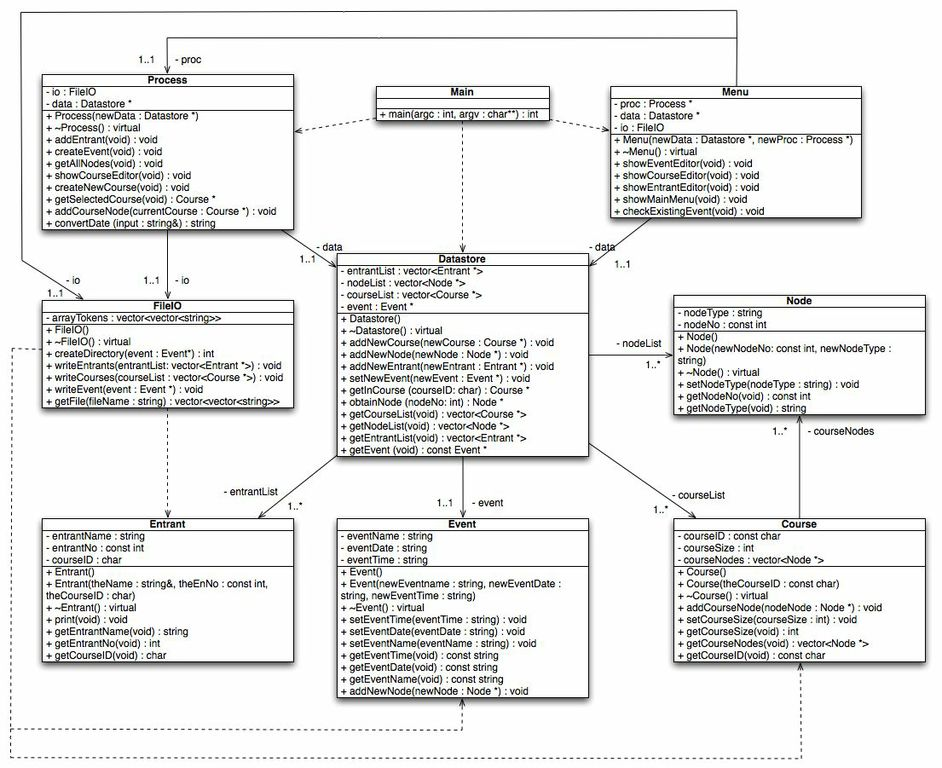
\includegraphics[scale=0.35]{event_creator_class_diagram.jpg}
\caption{UML class diagram detailing the structural design of the event creator application.}
\end{figure}

\clearpage
\subsection{Checkpoint Manager (Java)}

This application uses a structural design not too dissimilar to that of the event creator application. Three ``model" classes (\textit{Entrant, Course, Node}) and a shared \textit{Datastore} class form the data model for the application, and the \textit{ProcessData} class provides the core processing/functionality for the application. A public ENUM class (\textit{Datatype}) is used to differentiate between the data types processed by the system. \\\\
The GUI consists of a `JFrame' \textit{GUIFrame} class (window) and a `JPanel' \textit{GUIPanel} class (content) that interacts with the \textit{Datastore}, \textit{ProcessData} and \textit{FileIO} classes to allow the user to interact with the system and add new checkpoint times. The majority of error checking and exception handling occurs within the \textit{GUIPanel} class.

\begin{figure}[ht!]
\centering
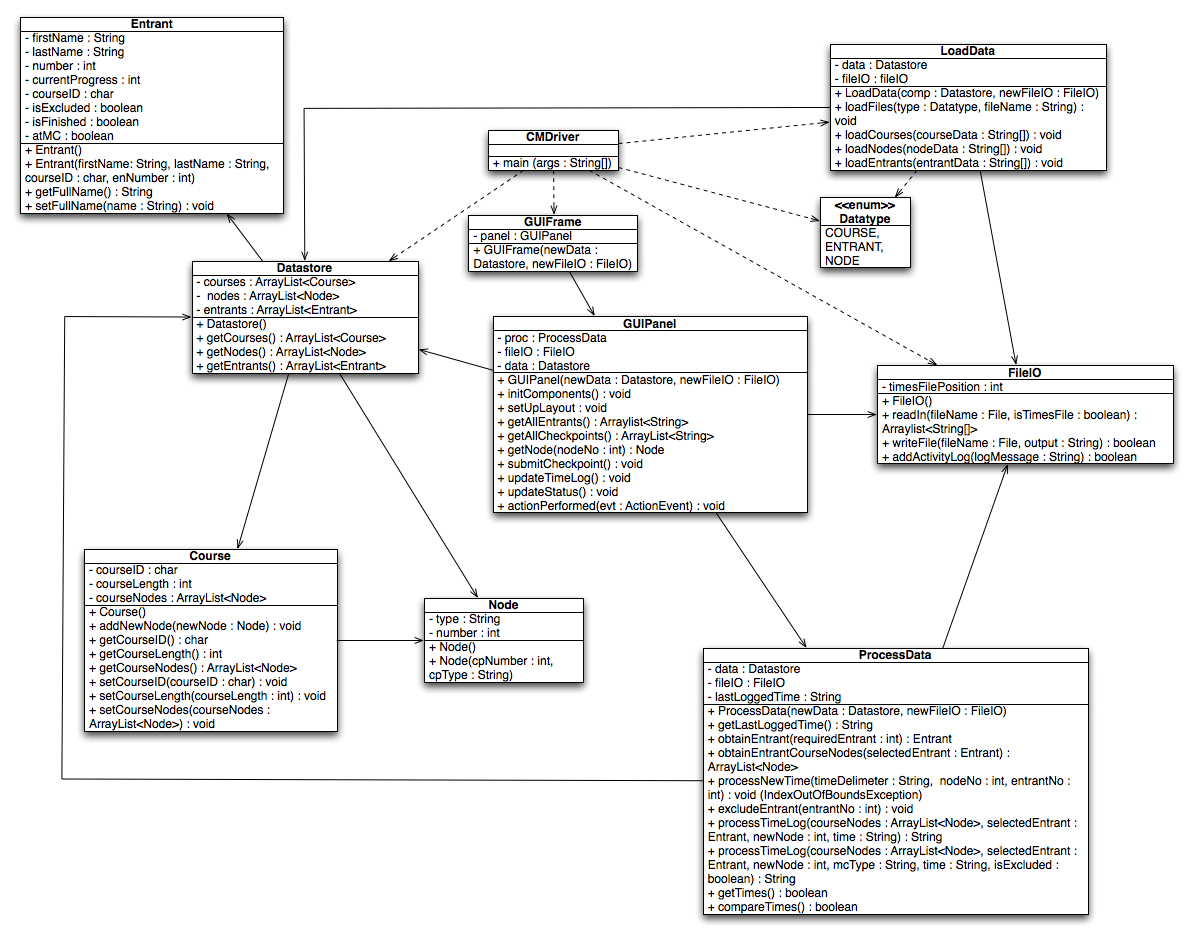
\includegraphics[scale=0.35]{checkpoint_manager_class_diagram.jpg}
\caption{Checkpoint Manager GUI informing user that entrant 98 must have arrived at a MC before they can depart.}
\end{figure}

\subsection{Event Manager (C)}

The event manager application is almost identical to that of the 'extended mission' application produced for CS23710, with the addition of file writing and file locking operations which allow the system to log user activity to an external file. \\\\
Apart from the addition of logging functions, and the removal of the ability to manually enter in checkpoint times (now the responsibility of the checkpoint manager application) no major changes have been made to the original application. 

\addcontentsline{toc}{section}{References}
\bibliographystyle{plain}

\begin{thebibliography}{1}

  \bibitem{notes} N. Snooke, D. Price, F. Labrosse {\em ``CS22510 Assignment One, 2012-2013 Runners and Riders - ``Out and about"} 2013: Aberystwyth University, Aberystwyth.
 
 \bibitem{notes} {\em ``How to lock files in C/C++ using fopen"}  - http://stackoverflow.com/questions/7573282/ 2011: StackOverflow, StackExchange.
 
  \bibitem{notes} {\em ``Demonstrates file locking and simple file read and write operations using java.nio.channels.FileChannel"}  - http://java2s.com/Code/Java/File-Input-Output/DemonstratesfilelockingandsimplefilereadandwriteusingjavaniochannelsFileChannel .htm 2011: Java2s.com, 12 Demo Source and Support.
 
  \bibitem{notes} P. Prinz, T. Crawford {\em ``C in a Nutshell"} 2008: O'Reilly Media Inc.
  
  \bibitem{notes} R. Lischner {\em ``C++ in a Nutshell"} 2009: O'Reilly Media Inc.
  
\end{thebibliography}

\end{document}